% Options for packages loaded elsewhere
\PassOptionsToPackage{unicode}{hyperref}
\PassOptionsToPackage{hyphens}{url}
\PassOptionsToPackage{dvipsnames,svgnames,x11names}{xcolor}
%
\documentclass[
]{article}
\usepackage{amsmath,amssymb}
\usepackage{iftex}
\ifPDFTeX
  \usepackage[T1]{fontenc}
  \usepackage[utf8]{inputenc}
  \usepackage{textcomp} % provide euro and other symbols
\else % if luatex or xetex
  \usepackage{unicode-math} % this also loads fontspec
  \defaultfontfeatures{Scale=MatchLowercase}
  \defaultfontfeatures[\rmfamily]{Ligatures=TeX,Scale=1}
\fi
\usepackage{lmodern}
\ifPDFTeX\else
  % xetex/luatex font selection
\fi
% Use upquote if available, for straight quotes in verbatim environments
\IfFileExists{upquote.sty}{\usepackage{upquote}}{}
\IfFileExists{microtype.sty}{% use microtype if available
  \usepackage[]{microtype}
  \UseMicrotypeSet[protrusion]{basicmath} % disable protrusion for tt fonts
}{}
\makeatletter
\@ifundefined{KOMAClassName}{% if non-KOMA class
  \IfFileExists{parskip.sty}{%
    \usepackage{parskip}
  }{% else
    \setlength{\parindent}{0pt}
    \setlength{\parskip}{6pt plus 2pt minus 1pt}}
}{% if KOMA class
  \KOMAoptions{parskip=half}}
\makeatother
\usepackage{xcolor}
\usepackage[margin=1in]{geometry}
\usepackage{longtable,booktabs,array}
\usepackage{calc} % for calculating minipage widths
% Correct order of tables after \paragraph or \subparagraph
\usepackage{etoolbox}
\makeatletter
\patchcmd\longtable{\par}{\if@noskipsec\mbox{}\fi\par}{}{}
\makeatother
% Allow footnotes in longtable head/foot
\IfFileExists{footnotehyper.sty}{\usepackage{footnotehyper}}{\usepackage{footnote}}
\makesavenoteenv{longtable}
\usepackage{graphicx}
\makeatletter
\def\maxwidth{\ifdim\Gin@nat@width>\linewidth\linewidth\else\Gin@nat@width\fi}
\def\maxheight{\ifdim\Gin@nat@height>\textheight\textheight\else\Gin@nat@height\fi}
\makeatother
% Scale images if necessary, so that they will not overflow the page
% margins by default, and it is still possible to overwrite the defaults
% using explicit options in \includegraphics[width, height, ...]{}
\setkeys{Gin}{width=\maxwidth,height=\maxheight,keepaspectratio}
% Set default figure placement to htbp
\makeatletter
\def\fps@figure{htbp}
\makeatother
\setlength{\emergencystretch}{3em} % prevent overfull lines
\providecommand{\tightlist}{%
  \setlength{\itemsep}{0pt}\setlength{\parskip}{0pt}}
\setcounter{secnumdepth}{5}
% definitions for citeproc citations
\NewDocumentCommand\citeproctext{}{}
\NewDocumentCommand\citeproc{mm}{%
  \begingroup\def\citeproctext{#2}\cite{#1}\endgroup}
\makeatletter
 % allow citations to break across lines
 \let\@cite@ofmt\@firstofone
 % avoid brackets around text for \cite:
 \def\@biblabel#1{}
 \def\@cite#1#2{{#1\if@tempswa , #2\fi}}
\makeatother
\newlength{\cslhangindent}
\setlength{\cslhangindent}{1.5em}
\newlength{\csllabelwidth}
\setlength{\csllabelwidth}{3em}
\newenvironment{CSLReferences}[2] % #1 hanging-indent, #2 entry-spacing
 {\begin{list}{}{%
  \setlength{\itemindent}{0pt}
  \setlength{\leftmargin}{0pt}
  \setlength{\parsep}{0pt}
  % turn on hanging indent if param 1 is 1
  \ifodd #1
   \setlength{\leftmargin}{\cslhangindent}
   \setlength{\itemindent}{-1\cslhangindent}
  \fi
  % set entry spacing
  \setlength{\itemsep}{#2\baselineskip}}}
 {\end{list}}
\usepackage{calc}
\newcommand{\CSLBlock}[1]{\hfill\break\parbox[t]{\linewidth}{\strut\ignorespaces#1\strut}}
\newcommand{\CSLLeftMargin}[1]{\parbox[t]{\csllabelwidth}{\strut#1\strut}}
\newcommand{\CSLRightInline}[1]{\parbox[t]{\linewidth - \csllabelwidth}{\strut#1\strut}}
\newcommand{\CSLIndent}[1]{\hspace{\cslhangindent}#1}
\usepackage{caption} \usepackage{setspace}\doublespacing \usepackage{lineno} \linenumbers \newcommand{\beginsupplement}{\setcounter{table}{0} \renewcommand{\thetable}{S\arabic{table}} \setcounter{figure}{0} \renewcommand{\thefigure}{S\arabic{figure}}}
\usepackage{booktabs}
\usepackage{longtable}
\usepackage{array}
\usepackage{multirow}
\usepackage{wrapfig}
\usepackage{float}
\usepackage{colortbl}
\usepackage{pdflscape}
\usepackage{tabu}
\usepackage{threeparttable}
\usepackage{threeparttablex}
\usepackage[normalem]{ulem}
\usepackage{makecell}
\usepackage{xcolor}
\ifLuaTeX
  \usepackage{selnolig}  % disable illegal ligatures
\fi
\usepackage{bookmark}
\IfFileExists{xurl.sty}{\usepackage{xurl}}{} % add URL line breaks if available
\urlstyle{same}
\hypersetup{
  pdftitle={Binocular combination in the autonomic nervous system},
  colorlinks=true,
  linkcolor={black},
  filecolor={Maroon},
  citecolor={Blue},
  urlcolor={Blue},
  pdfcreator={LaTeX via pandoc}}

\title{Binocular combination in the autonomic nervous system}
\author{Federico G. Segala\(^1\), Aurelio Bruno\(^{1,2}\), Joel T. Martin\(^{1,3}\),\\
Anisa Y. Morsi\(^1\), Alex R. Wade\(^{1,4}\) \& Daniel H. Baker\(^{1,4}\)}
\date{}

\begin{document}
\maketitle

\(^1\)Department of Psychology, University of York, Heslington, York, YO10 5DD, United Kingdom.

\(^2\)School of Psychology and Vision Sciences, University of Leicester, Leicester, LE1 7RH, United Kingdom.

\(^3\)School of Philosophy, Psychology and Language Sciences, University of Edinburgh, Edinburgh, EH8 9AD, United Kingdom.

\(^4\)York Biomedical Research Institute, University of York, Heslington, York, YO10 5NG, United Kingdom.

Corresponding author: Federico G. Segala, \url{federico.segala@york.ac.uk}.

Number of pages: 21

Number of figures: 4

Number of tables: 1

Number of words for abstract: 187/250

Number of words for introduction: 634/650

Number of words for discussion: 600/1500

Conflict of interest: The authors declare no competing financial interests.

Acknowledgements: Supported by Biotechnology and Biological Sciences Research Council grant BB/V007580/1 awarded to DHB and ARW.

\pagebreak

\section{Abstract}\label{abstract}

Pupil diameters are regulated by the autonomic nervous system, which combines light signals across the eyes independently of the visual cortex. Distinct classes of retinal photoreceptor are involved in this process, with cones and rods driving the initial constriction and intrinsically photosensitive retinal ganglion cells maintaining diameter over prolonged time periods. We investigated binocular combination by targeting different photoreceptor pathways using a novel binocular multiprimary system to modulate the input spectra via silent substitution. At the first harmonic of the modulation frequency, light flux and S-cone responses showed strong binocular facilitation, and weak interocular suppression. Melanopsin responses were invariant to the number of eyes stimulated. Notably, the L-M pathway involved binocular inhibition, whereby responses to binocular stimulation were weaker than for monocular stimulation. The second harmonic involved strong interocular suppression in all pathways, but with some evidence of binocular facilitation. Our results are consistent with a computational model of binocular signal combination (implemented in a Bayesian hierarchical framework), in which the weight of interocular suppression differs across pathways. We also find pathway differences in response phase, consistent with different lag times for phototransduction. This work demonstrates for the first time the algorithm governing binocular combination in the autonomic nervous system.

\section{Significance statement}\label{significance-statement}

Pupil diameters are determined by a network of subcortical nuclei that must combine incoming light levels across the two eyes, independently of cortical visual areas. We investigated the algorithmic properties of this binocular combination process for the first time. Using silent subsitution, we targeted different post-retinal pathways (light flux, L-M cones, S-cones, and melanopsin) with flickering stimuli generated by a novel binocular multi-primary system. We found different patterns of binocular combination across pathways, and also differences in the phase of the pupil response. The results were well described by a computational model of binocular signal combination, in which the weight of suppression between the eyes differed across pathways. This elucidates the algorithm governing binocular combination in the autonomic nervous system.

\section{Introduction}\label{introduction}

The autonomic nervous system regulates many involuntary bodily processes, including the constriction and dilation of the pupils in response to light (\citeproc{ref-McDougal2015}{McDougal and Gamlin, 2015}). The anatomical pathway from the retina to the subcortical nuclei controlling the pupillary light response (PLR) is well established: it includes the Pretectal Olivary nucleus (PON), the Superior Cervical ganglion and the Edinger-Westphal nucleus, which project to the iris sphincter muscles that directly control the pupil size (\citeproc{ref-McDougal2015}{McDougal and Gamlin, 2015}). Evidence of a binocular component to the PLR is shown by the consensual response of the pupil (stimulation of one eye will cause constriction of the other eye; \citeproc{ref-Wyatt1981}{Wyatt and Musselman, 1981}). The anatomical segregation of the subcortical pathway from the rest of the brain means that this binocular combination of signals must occur independently of the cortical processes of binocular integration required for visual perception. Our recent work (\citeproc{ref-Segala2023}{Segala et al., 2023}) has shown that the algorithm underlying binocular combination of light in the pupil pathway differs from that in the cortex. Here we extend this paradigm to compare binocular combination in different photoreceptor pathways that feed into the autonomic nervous system.

Different classes of retinal photoreceptors, including cones, rods and melanopsin-containing intrinsically photosensitive retinal ganglion cells (ipRGCs), are directly involved in controlling and maintaining the size of the pupils (e.g. \citeproc{ref-McDougal2010}{McDougal and Gamlin, 2010}; \citeproc{ref-Spitschan2014}{Spitschan et al., 2014}; \citeproc{ref-Barrionuevo2016}{Barrionuevo and Cao, 2016}; \citeproc{ref-Murray2018}{Murray et al., 2018}; \citeproc{ref-Woelders2018}{Woelders et al., 2018}). Cones drive the initial rapid constriction of the pupils (\citeproc{ref-Mathot2018}{Mathôt, 2018}), while the slower and longer activation of the ipRGCs maintains constriction over a prolonged period of time and regulates the post-illumination pupillary response (\citeproc{ref-Markwell2010}{Markwell et al., 2010}; \citeproc{ref-McDougal2010}{McDougal and Gamlin, 2010}). The ipRGCs are a recently discovered photoreceptor class (\citeproc{ref-Provencio2000}{Provencio et al., 2000}) that express the photopigment melanopsin, and are involved in the regulation of the circadian rhythm (\citeproc{ref-Panda2002}{Panda et al., 2002}; \citeproc{ref-Ruby2002}{Ruby et al., 2002}), forming a major input to the PON (\citeproc{ref-Dacey2003}{Dacey et al., 2003}). The first direct evidence of the involvement of the ipRGCs in the PLR was shown in melanopsin knockout rats by Lucas et al. (\citeproc{ref-Lucas2003}{2003}), resulting in the loss of the intrinsic photosensitivity of the cells and a reduced pupil constriction. Similar behaviour was later observed in primates and humans (\citeproc{ref-Gamlin2007}{Gamlin et al., 2007}) using silent substitution (see Methods), where it was demonstrated that the PLR continues during light presentation even when cone and rod signalling is blocked, indicating the primary role of the ipRGCs in maintaining pupil constriction over a prolonged time.

Binocular combination has been extensively studied in visual perception, where it is mediated by neurons in primary visual cortex (\citeproc{ref-Hubel1962}{Hubel and Wiesel, 1962}). For pattern vision, binocular summation occurs at threshold, such that a lower contrast is required to detect a target shown to both eyes than a target shown to one eye (\citeproc{ref-Campbell1965}{Campbell and Green, 1965}; \citeproc{ref-Baker2018}{Baker et al., 2018}). At higher contrasts, the phenomenon of `ocularity invariance' is observed, in which the response to monocularly- and binocularly-presented patterns is equal (\citeproc{ref-Baker2007}{Baker et al., 2007}; \citeproc{ref-Moradi2009}{Moradi and Heeger, 2009}). This is explained by a process of interocular suppression that cancels out the additional excitatory drive caused by stimulating two eyes. Our recent work (\citeproc{ref-Segala2023}{Segala et al., 2023}) showed that cortical signal combination for luminance flicker is substantially more linear than for spatial patterns, whereas there is evidence of interocular suppression in the pupil pathway. Here we measure the amplitude of pupil modulations in response to flickering stimuli presented as light flux, or directed towards the L-M cone, S-cone, and melanopsin pathways (see Figure \ref{fig:spectraplots}e-l). Our key comparisons are between monocular and binocular stimulation, and in a dichoptic masking condition where the two eyes are stimulated at different frequencies. The results are interpreted using a contemporary model of binocular vision (\citeproc{ref-Meese2006}{Meese et al., 2006}) implemented within a hierarchical Bayesian framework.

\section{Materials and methods}\label{materials-and-methods}

\subsection{Participants}\label{participants}

Twenty-four participants were recruited for each of the four experiments for a total of ninety-six adult participants (28 male, 68 female), whose ages ranged from 18 to 41. All participants had normal or corrected to normal vision, no known abnormalities of binocular or colour vision, and gave written informed consent. Our procedures were approved by the Ethics Committee of the Department of Psychology at the University of York (identification number 184).

\subsection{Apparatus \& stimuli}\label{apparatus-stimuli}

To present synchronised stimulus modulations independently to each eye, two light engines (SpectraTuneLAB, which are thermally stable across time with active cooling according to the manufacturers: LEDMOTIVE Technologies, LLC, Barcelona, Spain), each with 10 independently addressable LED colour channels, were integrated into a customised binocular viewing system. The light engines were operated via a Python interface to their REST API (\citeproc{ref-Martin2022}{Martin et al., 2022}), which supports synchronous launch and playback of spectral sequences prepared in advance and stored in JSON format. A special command was commissioned from LEDMOTIVE to allow two different stimulus files to be launched simultaneously from the two devices. The synchronisation of the spectra from the two devices was tested and showed that they were synchronised to within approximately 3ms.

When preparing the spectral sequences, the age of participants was used to account for the yellowing of the lenses. We used the silent substitution technique (\citeproc{ref-Estevez1982}{Estévez and Spekreijse, 1982}) to selectively stimulate specific photoreceptor classes. Silent substitution exploits the fact that each photoreceptor class has a distinct spectral tuning that overlaps with the others. Using a multiprimary system, in which the primaries (i.e.~LEDs) have different spectra, it is possible to target one class of photoreceptors while maintaining the others at a constant activity level, effectively silencing them (\citeproc{ref-Shapiro1996}{Shapiro et al., 1996}; \citeproc{ref-Spitschan2018}{Spitschan and Woelders, 2018}, this paper also offers a clear explanation of how to implement silent substitution). We calculated silent substitution solutions using the \emph{PySilSub} toolbox (\citeproc{ref-Martin2023}{Martin et al., 2023}), using linear algebra. The outputs of the two light engines (see Figure \ref{fig:spectraplots}b,c) were calibrated using an Ocean Optics Jaz spectroradiometer, which was wavelength-calibrated to an Argon lamp and intensity calibrated using a NIST-traceable light source. Each primary was also linearized using a polynomial fit (see Figure \ref{fig:primarylinearity} for details). We used the Stockman and Sharpe (\citeproc{ref-Stockman2000}{2000}) 10-degree cone fundamentals, and estimates of melanopsin absorbance spectra from CIE S 026 (discussed in \citeproc{ref-Martin2023}{Martin et al., 2023}) to calculate \(\alpha\)-opic irradiance.

The output from the light engines was directed through liquid light guides (LLG3-8H: Thorlabs Ltd, Cambridgeshire, UK) and diffused onto semi-opaque and highly diffusive white glass discs with a diameter of 50 mm for even illumination (34-473: Edmund Optics, York, UK). The light guide gaskets were butt-coupled to the light engine diffusers with threaded adapters (SM1A9, AD3LLG: Thorlabs Ltd, Cambridgeshire, UK) and the exiting ends of the light guides were mated with 51 mm depth optical cylinders (SM2L20: Thorlabs Ltd, Cambridgeshire, UK) via appropriately threaded adapters (AD3LLG, SM2A6: Thorlabs Ltd, Cambridgeshire, UK). The stimulus diffuser discs were retained at the front end of the optical cylinders approximately 51 mm from the light source, at which distance the output beam was sufficiently dispersed to afford even illumination of the diffuser when viewed from the front. To guarantee safe illumination levels, a circular neutral-density filter with the same diameter of the white glass discs (50 mm) and an optical density of 0.6 log units was placed in the optical path between the light source and the diffusers. A small circular piece of blackout material with a diameter of approximately 8 degrees (10 mm) was positioned centrally on the front of each diffuser disc to aid as a fusion lock, as a fixation point, and to occlude the fovea.

The diffuser discs were positioned in the objective planes of the lenses of a modified VR headset (SHINECON SC-G01, Dongguan Shinecon Industrial Co.~Ltd., Guangdong, China), which was used by the participants to view the stimuli. The stimuli were two discs of flickering light with a diameter of approximately 30 degrees, which were fused together into a cyclopean percept resembling a donut-shaped ring of light, similar to that used in other studies (\citeproc{ref-Spitschan2014}{Spitschan et al., 2014}, \citeproc{ref-Spitschan2015}{2015}; e.g., \citeproc{ref-Barrionuevo2016}{Barrionuevo and Cao, 2016}; \citeproc{ref-Murray2018}{Murray et al., 2018}; \citeproc{ref-Zele2018}{Zele et al., 2018}). The VR headset modifications allowed for small adjustments to account for individual differences in interpupillary distance and focal length. The use of this set up allowed us to modulate the stimuli in three different ocular configurations, similar to the ones we used in our previous study (\citeproc{ref-Segala2023}{Segala et al., 2023}): monocular, binocular and dichoptic. In the monocular configuration, the unstimulated eye still saw a non-flickering disc of mean light flux. A schematic of the stimulation system is shown in Figure \ref{fig:spectraplots}a. Pupillometry data were collected using a binocular Pupil Core eye-tracker headset (Pupil Labs GmbH, Berlin, Germany, \citeproc{ref-Kassner2014}{Kassner et al., 2014}) running at 120 Hz, and the signals were recorded with the Pupil Capture software.

Our previous study (\citeproc{ref-Segala2023}{Segala et al., 2023}) used a temporal frequency of 2Hz for foveal luminance flicker, and recorded EEG data simultaneously with pupillometry. Initial pilot experiments indicated that this frequency was too high to elicit measurable responses when stimulating individual photoreceptor pathways. For all experiments, we therefore used a primary flicker frequency of 0.5Hz, as previous literature showed that this was slow enough to elicit a pupil response from all photoreceptor classes (\citeproc{ref-Spitschan2014}{Spitschan et al., 2014}). We also focussed on only recording pupillometry data as this frequency would be too slow to elicit steady-state EEG responses (\citeproc{ref-Norcia2015}{Norcia et al., 2015}).

For all experiments, sinusoidal temporal modulations were presented against the same background spectrum (matched between the eyes), which was used to achieve silent substitution in the three photoreceptor modulation experiments. The background spectra were defined by setting all channels to half maximum output for the brighter of the two devices (STLab 1, left eye) and then using the STLab 1/STLab 2 calibration ratio to find the equivalent settings for the companion device (STLab 2, right eye). The background spectrum illuminance was approximately 74 lux, or 68.5 cd/m\(^2\). The spectral power distributions and \(\alpha\)-opic irradiances of the background spectra for both eyes are shown in Figure \ref{fig:spectraplots}c-d.

Silent substitution stimuli were prepared and calibrated for each participant with custom Python software (\citeproc{ref-Martin2023}{Martin et al., 2023}) and Python scripts. Estimates of photoreceptor spectral sensitivities for each participant were constructed from the known photopigment absorbance spectra (\citeproc{ref-Stockman2000}{Stockman and Sharpe, 2000}), taking account of the peak axial density of the respective photopigments, as well as lens (\citeproc{ref-Pokorny1987}{Pokorny et al., 1987}; \citeproc{ref-Stockman1999}{Stockman et al., 1999}; \citeproc{ref-Stockman2000}{Stockman and Sharpe, 2000}) and macular pigment density (\citeproc{ref-Bone1988}{Bone et al., 1988}; \citeproc{ref-Stockman1999}{Stockman et al., 1999}), in accordance with the field size and age-dependant CIEPO06 observer model (\citeproc{ref-CIE2006}{CIE, 2006}). The melanopic and rhodopic action spectra of the 32-year-old standard observer were taken from CIE S 026 (\citeproc{ref-CIE2018}{CIE, 2018}) and then adjusted for age-related lens transmittance with a spectral correction function, in line with the standard. Macular pigment correction was not applied to the rhodopic and melanopic action spectra because rods are not present at the fovea and ipRGCs sit above the retinal pigment layer (\citeproc{ref-Trieschmann2007}{Trieschmann et al., 2007}).

In the light flux experiment, the stimulus intensity was increased and decreased relative to the background, which we expected to modulate all photoreceptor classes (see Figure \ref{fig:spectraplots}e,i). In the L-M cone modulation experiment, we used silent substitution to increase the L-cone activity, and simultaneously decrease the M-cone activity, during the first half-cycle of the sine wave. In the second half-cycle the polarity of the modulation reversed (see Figure \ref{fig:spectraplots}f,j). The maximum available L-M contrast was approximately 10\%. In the S-cone modulation experiment, we increased and decreased S-cone-directed signals, whilst keeping activity in the other photoreceptors constant (see Figure \ref{fig:spectraplots}g,k). Our system allowed a maximum contrast of 45\%. Finally, in the melanopsin experiment, we modulated the activity of the melanopsin-containing intrinsically photoreceptive retinal ganglion cells, whilst keeping cone activity constant (see Figure \ref{fig:spectraplots}h,l). The maximum available melanopsin contrast was 22\%. We assume that the activity of rods was constant at the high background luminance intensity used here, and so did not attempt to silence rod activity in any condition, as this would have greatly reduced the available dynamic range. Splatter on nominally silenced photoreceptors was very small (see Figure \ref{fig:spectraplots}j-l), well below the levels that would be expected to generate measurable pupil modulations, although we can observe that the rods may not be saturated in the L-M and melanopsin-directed stimuli (Figure \ref{fig:spectraplots}j and \ref{fig:spectraplots}l) and could intrude in these two experiments. We also estimated activation of penumbral L and M cones (\citeproc{ref-Spitschan2015}{Spitschan et al., 2015}; \citeproc{ref-Barrionuevo2016}{Barrionuevo and Cao, 2016}; \citeproc{ref-Zele2019}{Zele et al., 2019}), which was minimal (\(\le 1.5%
\) contrast; less than splatter on the open-field cones) for melanopsin-directed stimuli. We note that the temporal frequency of our modulation (0.5Hz) is well below the range where penumbral cone activation can elicit visible percepts, and that such percepts fade after around 1 second (\citeproc{ref-Spitschan2015}{Spitschan et al., 2015}), and do not typically affect pupil responses (\citeproc{ref-Spitschan2014}{Spitschan et al., 2014}).

\subsection{Procedure}\label{procedure}

Before the start of each experiment, participants adjusted the objective planes of the lenses with the help of the experimenter until the stimulus was in focus and they perceived the two pieces of blackout material as one fused disc. Pupil responses to binocular temporal contrast modulations were examined in a factorial design that combined six ocular conditions and five temporal contrast levels: 6, 12, 24, 48 and 96\% of the available dynamic range. This design, similar to that used in our previous studies (\citeproc{ref-Baker2017}{Baker and Wade, 2017}; \citeproc{ref-Baker2020}{Baker et al., 2020}; \citeproc{ref-Segala2023}{Segala et al., 2023}), was applied in four separate experiments, each with a different mode of photoreceptor stimulation. In the first three conditions, the discs flickered at 0.5 Hz, in either a monocular, binocular or dichoptic arrangement. In the dichoptic condition the non-target eye saw a flickering fixed contrast of 48\% of the available dynamic range. In the remaining three conditions (the cross-frequency conditions) one eye's disc flickered at 0.4 Hz, and the other eye's disc flickered at 0.5 Hz. This included monocular responses at 0.4 Hz, as well as binocular (one eye sees each frequency at the target contrast) and dichoptic (target stimulus flickering at 0.5 Hz, mask contrast of 48\% at 0.4 Hz in the other eye) arrangements. We counterbalanced presentation of the target stimulus across the left and right eyes.

The experiments were conducted in a windowless room, in which the only source of light was the modified VR headset. The participants sat as close as possible to the VR headset, leaving enough space for the eye-tracker to record the eyes. Each experiment was carried out in a single session of around 45-60 minutes, divided into three blocks of 15-17 minutes each. In each block, there were a total of 60 trials lasting 15 seconds each (12s of stimulus presentation, followed by 3s of interstimulus interval). The participants were given no task other than look at the black fixation dot while trying to minimise their blinking during the presentation period. For all experiments other than the light flux condition, participants adapted to the unmodulated background luminance for two minutes before stimulation began.

Before the start of the L-M experiment, participants completed a luminance nulling perceptual calibration procedure in L-M cone space on an Iiyama \(\textrm{VisionMaster}^{\textrm{TM}}\) Pro 510 display (800 x 600 pixels, 60 Hz refresh rate). During the task, participants were presented with a disc flickering within the L-M cone space (between magenta and cyan). Using a trackball, participants adjusted the angle in cone space to find their subjective isoluminant point, which resulted in changing the flickering intensity of the stimulus until the amplitude of the flicker appeared to be minimised. The result was used to modify the requested contrasts during stimulus preparation so as to account for individual differences affecting perceived illuminance, principally the L:M cone ratio (\citeproc{ref-Carroll2002}{Carroll et al., 2002}; \citeproc{ref-Hofer2005}{Hofer et al., 2005}).

\subsection{Data analysis}\label{data-analysis}

The pupillometry data were analysed using the same method we used in our previous study (\citeproc{ref-Segala2023}{Segala et al., 2023}). The data were converted from mp4 videos to a csv text file using the Pupil Player software (\citeproc{ref-Kassner2014}{Kassner et al., 2014}), which estimated pupil diameter for each eye on each frame using a 3D model of the eyeball. The individual data were then loaded into R for analysis, where a ten-second waveform for each trial in each eye was extracted (excluding the first two seconds after stimulus onset). We interpolated across any dropped or missing frames to ensure regular and continuous sampling over time. The Fourier transform was calculated for each waveform, and all repetitions of each condition were pooled across eye and then averaged. Finally, data were averaged across all participants to obtain the group results. We used coherent averaging and at each stage we excluded data points with a Mahalanobis distance exceeding \(D\) = 3 from the complex-valued mean (\citeproc{ref-Baker2021}{Baker, 2021}). For monocular stimulation, we confirmed that the consensual response was equivalent to the response in the stimulated eye.

For all experiments, we used a bootstrapping procedure with \ensuremath{10^{4}} iterations to estimate standard errors across participants. All analysis and figure construction was conducted using a single R-script, available online, making this study fully computationally reproducible: \url{https://osf.io/gdvt4/}.

\subsection{Computational model and parameter estimation}\label{computational-model-and-parameter-estimation}

To quantitatively summarise our data, we used the same model described in our previous study (\citeproc{ref-Segala2023}{Segala et al., 2023}). The model has the same general form as the first stage of the contrast gain control model proposed by Meese et al. (\citeproc{ref-Meese2006}{2006}), but omits the second stage. For the previous model that we used (\citeproc{ref-Segala2023}{Segala et al., 2023}), the exponent of the numerator and denominator had fixed values of 2 and (implicitly) 1. Here, we allow these parameters (called \emph{p} and \emph{q}) to be free, in order to permit different shapes of contrast response function, e.g.~accelerating or saturating. The responses of the left eye and right eye channels are as follows:

\begin{equation}
\label{eq:respL}
resp_L = \frac{L^p}{Z + L^q + \omega R^q},
\end{equation}

\begin{equation}
\label{eq:respR}
resp_R = \frac{R^p}{Z + R^q + \omega L^q},
\end{equation}

\noindent where \emph{L} and \emph{R} are the contrast signals from the left and right eyes, \emph{p} and \emph{q} are exponents, \emph{Z} is a saturation constant that shifts the contrast-response function laterally, and \(\omega\) is the weight of suppression from the other eye.

The responses from the two eyes are then summed binocularly:

\begin{equation}
\label{eq:respB}
resp_B = R_{max}(resp_L + resp_R) + k,
\end{equation}

\noindent where \emph{k} is a noise parameter, and \(R_{max}\) scales the overall response amplitude.

The models were fit using a hierarchical Bayesian framework implemented in Stan (\citeproc{ref-Carpenter2017}{Carpenter et al., 2017}). The data for each photoreceptor type and response frequency was fit separately, for a total of 8 model fits. The prior for the \(\omega\) parameter was Gaussian, with a mean of 1 and standard deviation of 0.5. Priors for the other free parameters were also Gaussian, with mean values based on previous work (\citeproc{ref-Segala2023}{Segala et al., 2023}). We calculated over \ensuremath{10^{6}} posterior samples, and retained 10\% for plotting.

\section{Results}\label{results}

Figure \ref{fig:spectraplots}m-p shows averaged waveforms of pupil diameter in response to binocular stimulation. For light flux stimuli (Figure \ref{fig:spectraplots}m) a strong modulation is apparent at the stimulation frequency (0.5Hz), which is also clear in the Fourier amplitude spectrum (Figure \ref{fig:spectraplots}q). For binocular stimulation of the L-M pathway, S-cone pathway and melanopsin pathway, pupil modulations were less than 10\% of the amplitude of the light flux modulation (note the change in y-axis scale for the Fourier spectra), but still apparent at 0.5Hz in the Fourier spectra (Figure \ref{fig:spectraplots}n-p). We also observed a second harmonic response (at 1Hz) for all conditions, which was weaker than the first harmonic for light flux and melanopsin stimulation, but stronger for L-M and S-cone stimulation. The second harmonic is also apparent in the pupil waveforms shown in Figure \ref{fig:spectraplots}n-p.~Our main analysis therefore focuses on the amplitude of the pupil modulations at both the first and second harmonic frequencies across different stimulus conditions.

\begin{figure}

{\centering 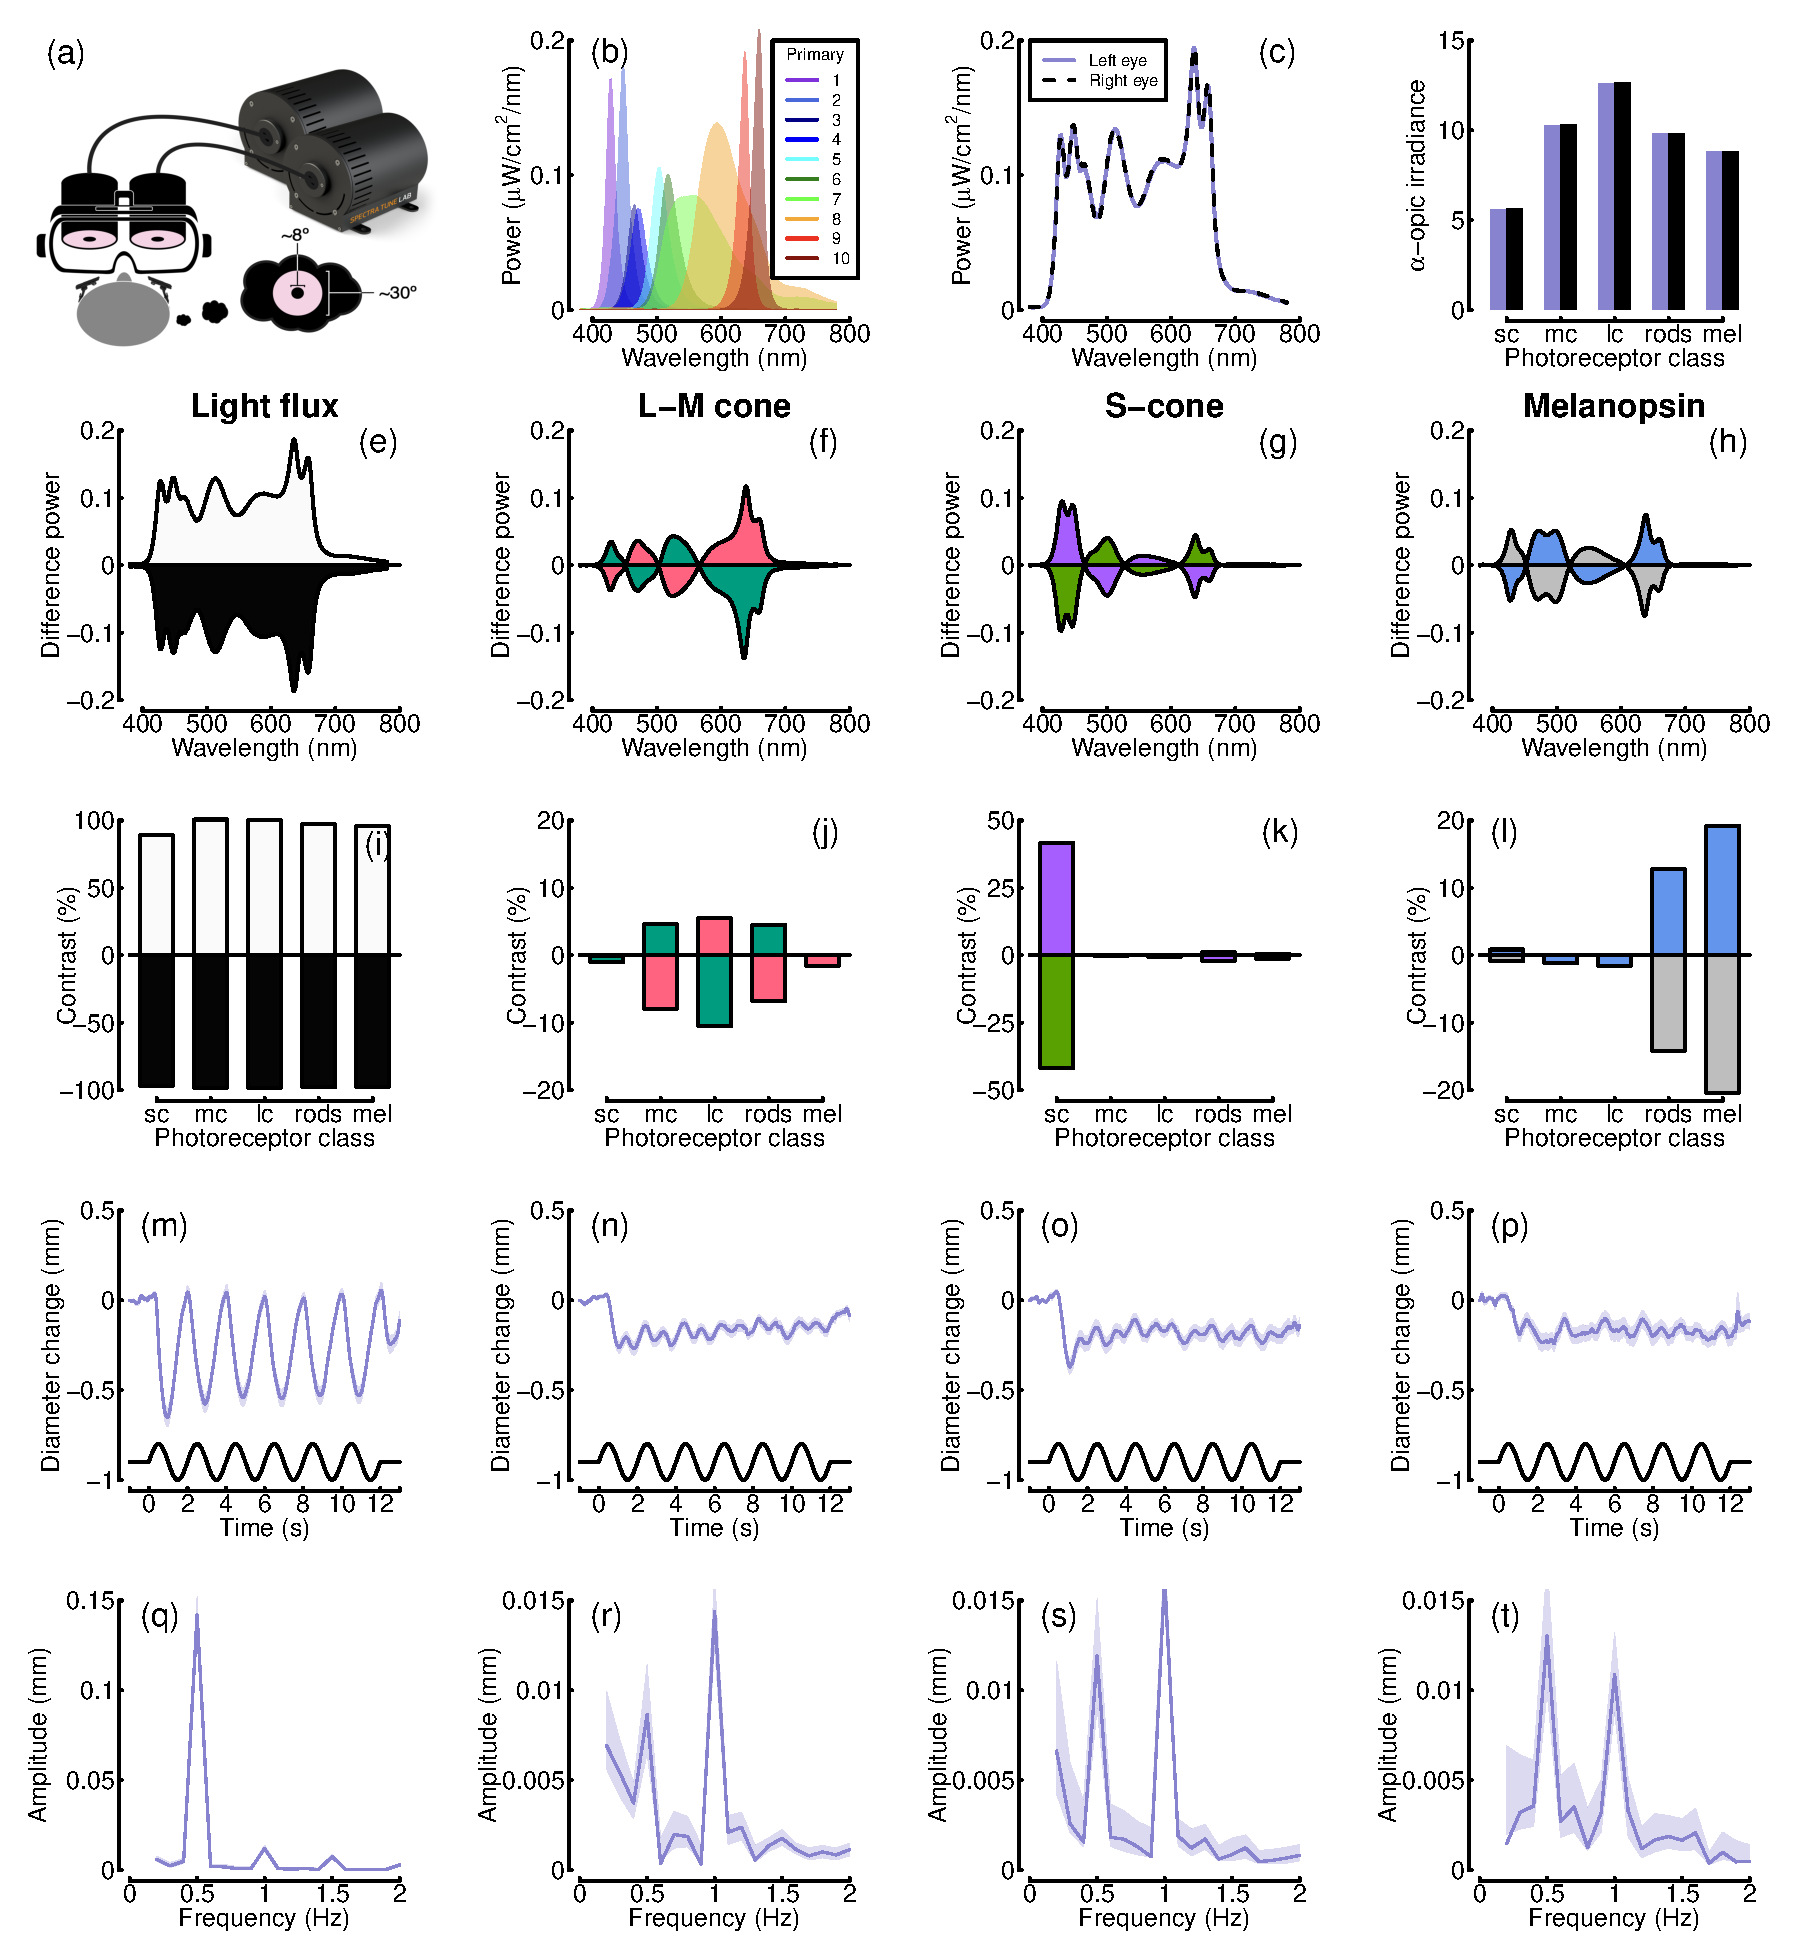
\includegraphics[width=0.8\linewidth]{Figures/methodsfigrods} 

}

\caption{Summary of the spectral power distributions and alpha-opic irradiances for the background and each condition, as well as averaged pupil diameters and Fourier spectra. Panel (a) shows a schematic of the binocular stimulation system for presenting spectrally tuned modulations independently to each eye. The VR headset was attached to a clamp stand that the experimenters could use to adjust the height and align the headset with the eyes of the participant. The participant's head was supported by a chin rest to keep it in position throughout the experiment. Panel (b) shows the outputs of each LED primary at maximum intensity, and panels (c) and (d) show the overall spectral power distributions and the alpha-opic irradiances of the background spectra used for both eyes. The subsequent rows show the power differences (e-h), and photoreceptor contrasts (i-l) relative to the background, averaged pupil diameter waveforms (m-p) and Fourier spectra (q-t) for binocular stimulation. Column headings indicate the pathway stimulated, and shaded regions in panels m-t indicate bootstrapped 95\% confidence intervals.}\label{fig:spectraplots}
\end{figure}

Figure \ref{fig:FirstHarmonicPlots}a-d shows contrast response functions across stimulation conditions for responses at the first harmonic of the main stimulation frequency (0.5Hz). In each plot, the response to monocular stimulation is given by the red circles and typically increases monotonically as a function of stimulus (temporal) contrast. Relative to monocular stimulation, binocular stimulation led to higher response amplitudes, indicating a binocular facilitation effect, for the light flux and S-cone conditions (Figure \ref{fig:FirstHarmonicPlots}a,c), and to some extent for the melanopsin condition (Figure \ref{fig:FirstHarmonicPlots}d). However, the L-M cone condition (Figure \ref{fig:FirstHarmonicPlots}b) produced a binocular suppression effect, where the response to binocular stimulation was weaker than the response to monocular stimulation (blue squares below red circles). These results indicate that the magnitude of binocular facilitation differs across photoreceptor pathway, suggesting heterogeneity in the underlying neural computation.

\begin{figure}

{\centering 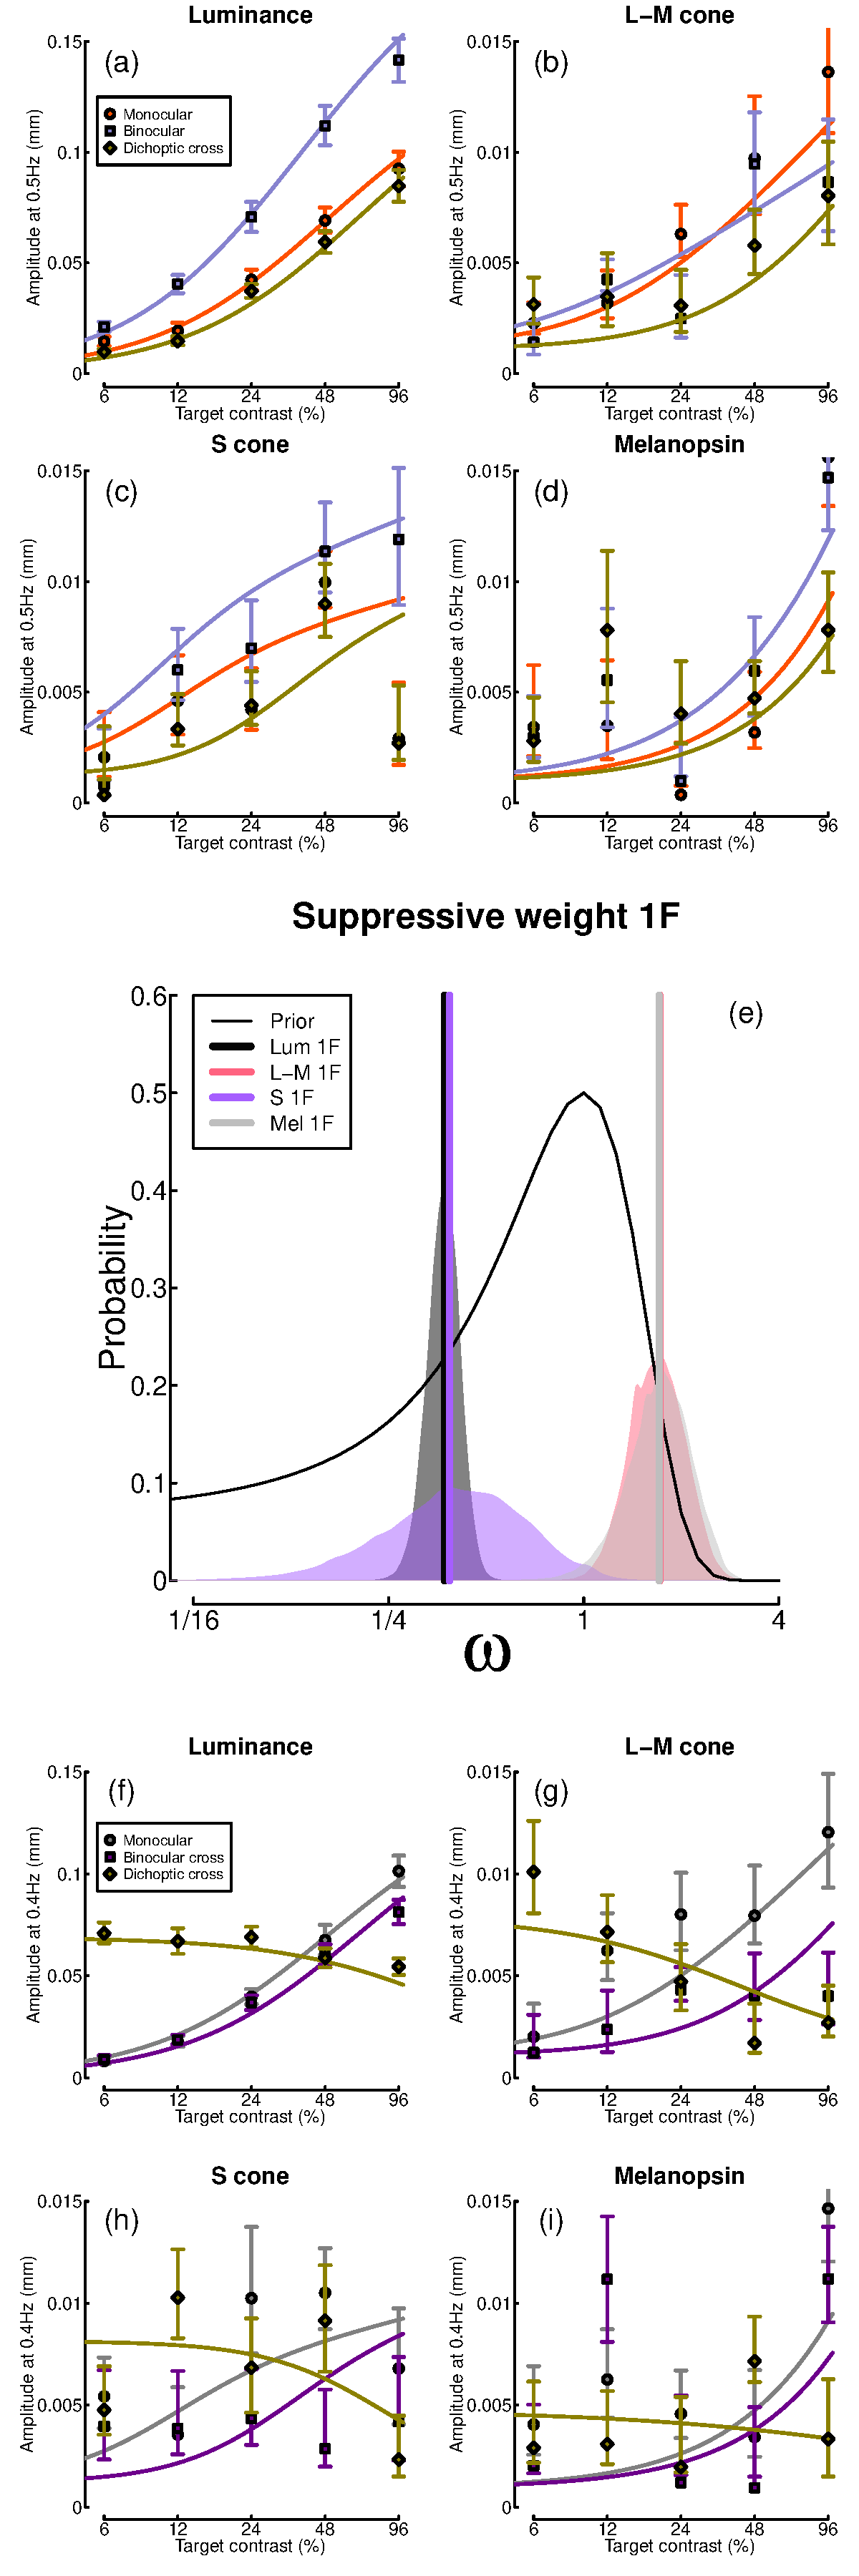
\includegraphics[width=0.4\linewidth]{Figures/FirstHarmonic} 

}

\caption{Contrast response functions for pupil modualations in response to flicker at 0.5Hz (panels a-d), and 0.4Hz (panels f-i), and posterior parameter distributions for the weight of interocular suppression (panel e). Within each panel (except panel e), data points are the coherently averaged amplitudes for each condition, and error bars indicate bootstrapped 95\% confidence intervals. Curves show model fits using the maximum a posteriori (MAP) parameter values (see Table 1). In panel (e), vertical lines show the MAP estimates, and the thin black curve indicates the prior (note the logarithmic x-axis).}\label{fig:FirstHarmonicPlots}
\end{figure}

In contemporary models of binocular signal combination, the amount of binocular facilitation is determined by the magnitude of interocular suppression, with strong suppression reducing facilitation (\citeproc{ref-Kingdom2015}{Kingdom and Libenson, 2015}). We can estimate the strength of interocular suppression by measuring how much monocular responses are reduced when a dichoptic `mask' is shown to the other eye. In our paradigm, the two components flickered at different frequencies (0.5 and 0.4Hz) so that their responses remained distinct in the Fourier spectrum (e.g. \citeproc{ref-Busse2009}{Busse et al., 2009}). The yellow diamond symbols in Figure \ref{fig:FirstHarmonicPlots}a-d show the target responses in this condition, and in most cases were weaker than the monocular responses (red circles). The strongest dichoptic masking is found in the L-M condition, where we also observed the binocular suppression effect. Suppression can also be estimated from the responses at 0.4Hz (Figure \ref{fig:FirstHarmonicPlots}f-i). The reduced amplitude in the binocular cross condition (where the two eyes received different temporal frequencies; purple squares) relative to the 0.4Hz monocular condition (grey circles), and the progressive decline in amplitude of the dichoptic cross response (yellow diamonds) also differ across photoreceptor conditions, showing similar differences to those observed at 0.5Hz.

To estimate the extent of interocular suppression for each photoreceptor pathway, we fitted each data set using a Bayesian hierarchical implementation of a simple binocular combination model (\citeproc{ref-Meese2006}{Meese et al., 2006}; \citeproc{ref-Segala2023}{Segala et al., 2023}). Our primary objective was to compare posterior distributions of the weight of interocular suppression, which are shown in Figure \ref{fig:FirstHarmonicPlots}e. Consistent with our earlier observations, the strongest suppressive weight corresponds to the L-M and Melanopsin conditions, and the weakest suppression corresponds to the light flux and S-cone conditions, with virtually no overlap between the posterior distributions for weak and strong suppression. The model fits were of good quality, as shown by the curves in Figure \ref{fig:FirstHarmonicPlots}a-d,f-i. The fitted model parameters are given in Table \ref{tab:paramtable}.

\begin{table}[H]

\caption{\label{tab:paramtable}Summary of maximum a posteriori (MAP) parameter estimates for each data set.}
\centering
\begin{tabular}[t]{lcccccc}
\toprule
Experiment & Z & k & w & p & q & Rmax\\
\midrule
Light flux 1F & 95.77 & 0.00083 & 0.37 & 1.32 & 1.24 & 0.0905\\
L-M cone 1F & 49.82 & 0.00109 & 1.71 & 1.50 & 1.21 & 0.0032\\
S cone 1F & 63.00 & 0.00121 & 0.39 & 1.94 & 1.79 & 0.0042\\
Melanopsin 1F & 79.61 & 0.00094 & 1.71 & 1.29 & 0.76 & 0.0025\\
\midrule
Light flux 2F & 48.81 & 0.00089 & 1.24 & 1.15 & 0.88 & 0.0039\\
L-M cone 2F & 66.00 & 0.00075 & 0.95 & 1.10 & 0.82 & 0.0050\\
S cone 2F & 75.94 & 0.00097 & 2.22 & 1.41 & 0.83 & 0.0018\\
Melanopsin 2F & 67.94 & 0.00101 & 1.37 & 0.90 & 0.49 & 0.0035\\
\bottomrule
\end{tabular}
\end{table}

At the second harmonic frequencies, the levels of suppression were more uniform across different photoreceptor pathways (see Figure \ref{fig:SecondHarmonicPlots}). In general, suppression estimates were near or above 1 (see lower rows of Table \ref{tab:paramtable}), with substantial overlap between the posterior distributions (Figure \ref{fig:SecondHarmonicPlots}e). The contrast response functions also looked more uniform, and generally involved less binocular facilitation and more interocular suppression than were seen at the first harmonics. The L-M condition now featured the weakest suppressive weight, and the strongest binocular facilitation, which was the opposite pattern seen at the first harmonic.

\begin{figure}

{\centering 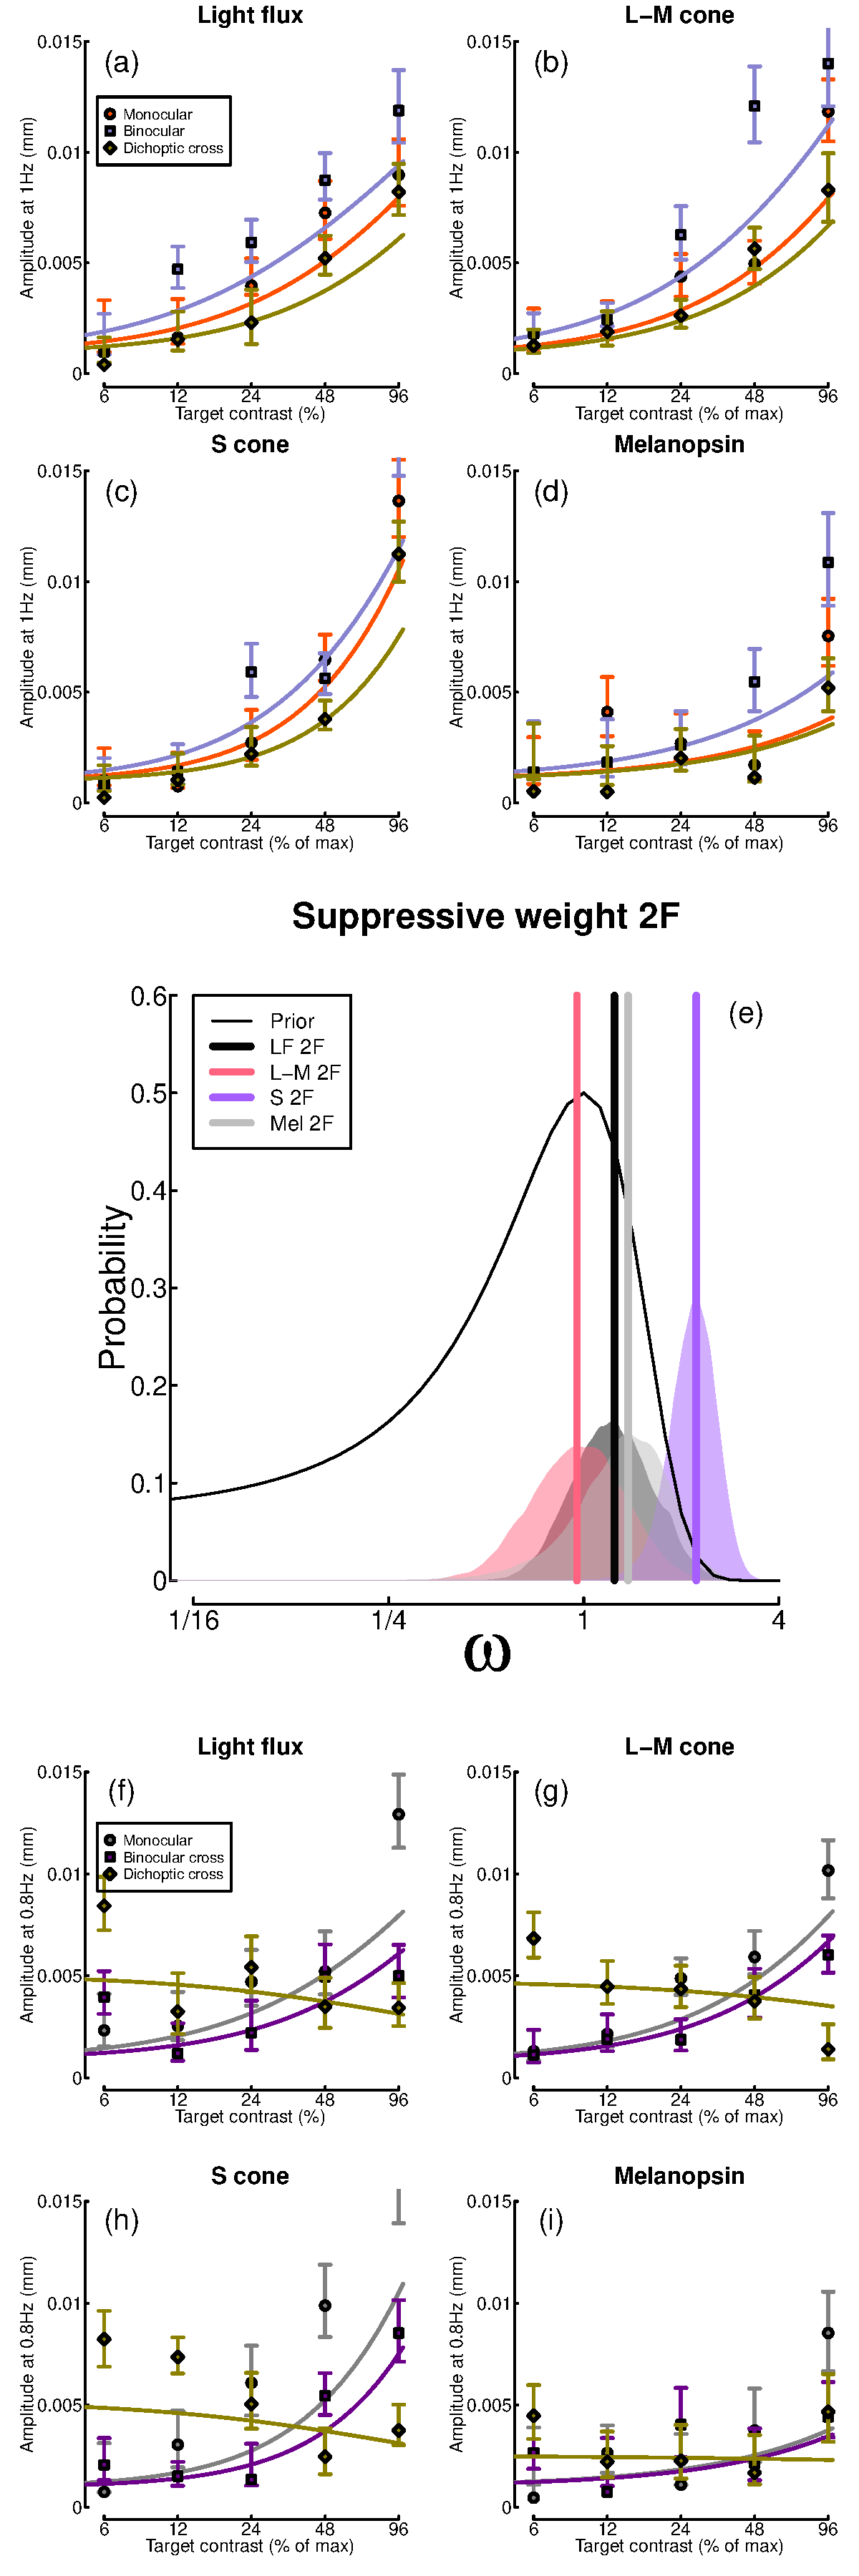
\includegraphics[width=0.4\linewidth]{Figures/SecondHarmonic} 

}

\caption{Responses at the second harmonic frequencies (1Hz and 0.8Hz), in the same format as Figure 2.}\label{fig:SecondHarmonicPlots}
\end{figure}

Finally, we inspected the response phase of our four stimulation conditions, given previous reports that these differ across pathways (\citeproc{ref-Spitschan2014}{Spitschan et al., 2014}), and may be in antiphase for melanopsin and S-cone signals. Figure \ref{fig:phaseplots} shows the phase angles for the first (a) and second (b) harmonic frequencies for binocular stimulation (monocular stimulation produced very similar results). At the first harmonic, melanopsin and S-cone signals differed in phase by more than 90 degrees, though they were not fully in antiphase. The light flux and L-M responses were approximately in antiphase to each other, however this is likely due to our choice to modulate L+M- in the first half-cycle of the sine wave (corresponding to a luminance increase in the light flux condition), and L-M+ in the second half-cycle (corresponding to a luminance decrease in the light flux condition). Had we reversed this phase arrangement, we would likely have seen a close phase correspondence between the L-M and light flux conditions (another way to think about this is that L-cone decreases and M-cone increases are processed like luminance increases). Phase differences between the light flux, S-cone and melanopsin conditions are likely attributable to different lags in phototransduction at the earliest stage (i.e.~in the retina). At the second harmonic frequency (Figure \ref{fig:phaseplots}b), the light flux condition was again out of phase with the other three, and was approximately in quadrature phase with the L-M condition, and in antiphase with both the S-cone and melanopsin conditions (which were in phase with each other). We note that the marked phase differences between conditions make the possibility that our results are dominated by rod activity relatively unlikely (e.g.~in the L-M and melanopsin conditions, which have very different phase profiles).

\begin{figure}

{\centering 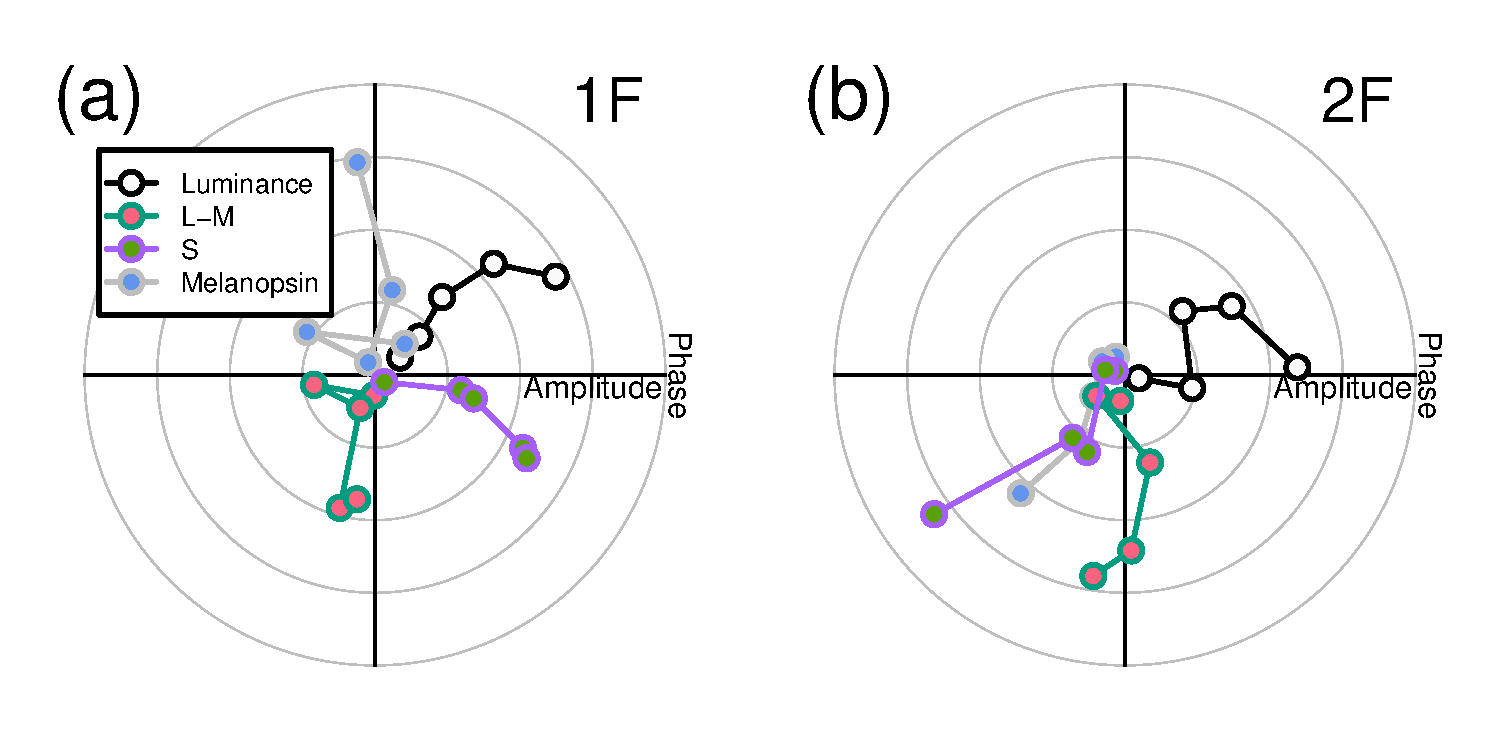
\includegraphics{Figures/phaseplots} 

}

\caption{Pupil phase plots at the first and second harmonic frequencies for the light flux, melanopsin, L-M pathway and the S-cone pathway conditions. Panel (a) shows the pupil response at the first harmonic frequency during binocular stimulation. Panel (b) shows the pupil response at the second harmonic frequency during binocular stimulation. The five data points for each pathway correspond to the five contrast levels displayed. In panel (a) the light flux amplitudes have been scaled down by a factor of 10 to enable comparison with the other conditions.}\label{fig:phaseplots}
\end{figure}

\section{Discussion}\label{discussion}

We used binocular pupillometry and silent substitution to measure monocular and binocular responses of the pupils to flickering stimuli when stimulating specific photoreceptor pathways. In all four experiments, we were able to record contrast response functions at both the first and the second harmonic frequencies. All experiments showed that binocular combination in the autonomic nervous system happens in a non-linear manner, with evidence of different magnitudes of interocular suppression depending on the photoreceptor pathway. This pattern of results was confirmed by a computational model, which allowed us to compare the weight of interocular suppression for each pathway. We found that at the first harmonic frequency the L-M and melanopsin pathways involved strong suppression, whereas the light flux and S-cone pathways involved weaker suppression. Suppression was strong in all four pathways at the second harmonic frequency. Finally, the phase of the pupil response revealed different lag times for the different pathways at the first and second harmonic frequencies.

This is the first study to investigate binocular interactions in the melanopsin pathway directly. A previous meta-analysis (\citeproc{ref-Spitschan2019}{Spitschan and Cajochen, 2019}) indicated that there may be a substantial binocular facilitation effect in the circadian pathway, as indexed by melatonin suppression (melatonin is a hormone released by the pineal gland; its production is suppressed by exposure to bright light, particularly when the melanopsin-containing ipRGCs are stimulated). In brief, monocular stimulation of the ipRGCs requires up to ten times the signal strength to produce an equivalent effect to binocular stimulation. This superadditive effect implies an absence of interocular suppression, and perhaps the presence of either a highly compressive nonlinearity, or an AND-style neural operation. Our findings here are very different - we do not see substantial binocular facilitation effects in response to melanopsin modulation, and our data indicate that interocular suppression is very strong. Moreover, by measuring the full contrast response function, we can rule out compressive nonlinearities, because the functions accelerate at both the first and second harmonic frequencies. The explanation for this difference could be due to different anatomical pathways. Binocular combination in the circadian system likely takes place in the suprachiasmatic nucleus, whereas in the pupil constriction circuit the Edinger-Westphal nucleus is the most likely site of binocular integration (\citeproc{ref-Mathot2018}{Mathôt, 2018}). Presumably these anatomical differences, and the practical constraints of the two systems, lead to differences in response.

Our recent psychophysical work (\citeproc{ref-Baker2024}{Baker et al., 2024}) has looked at binocular interactions in the L-M and S-cone pathways, and compared these to the light flux pathway. Using a contrast discrimination paradigm with spatial modulations of light flux and colour, Baker et al. (\citeproc{ref-Baker2024}{2024}) found equally strong interocular suppression in all three pathways. This is rather different from our pupillometry results here, which demonstrate weaker suppression in the light flux and S-cone pathways than in the L-M pathway (see Figure \ref{fig:FirstHarmonicPlots}). However, the current experiments involve temporal modulations, which are quite distinct from the spatial modulations used in Baker et al. (\citeproc{ref-Baker2024}{2024}). Our other recent work (\citeproc{ref-Segala2023}{Segala et al., 2023}) has shown that temporal luminance modulations involve much weaker interocular suppression in the cortical response than do spatial luminance modulations (\citeproc{ref-Baker2017}{Baker and Wade, 2017}). These different normalization processes might reflect different priorities for spatial and temporal vision. Spatial vision aims to fuse images to provide binocular single vision, and benefits from `ocularity invariance' (\citeproc{ref-Baker2007}{Baker et al., 2007}), in which visual appearance is constant when viewed with one eye or two. Temporal vision is critical for motion perception, which can involve alternative binocular computations, such as calculating velocity differences between the eyes (\citeproc{ref-Kaestner2019}{Kaestner et al., 2019}). Of course the present measurements were of pupil size, which may be subject to different anatomical and functional constraints from those in the cortex. Future research should aim to extend our current findings to perception using psychophysical approaches.

\section{Conclusions}\label{conclusions}

We have demonstrated that binocular combination of temporal flickering light in the autonomic nervous system depends on the photoreceptor pathway stimulated. We were able to elicit pupil responses by stimulating the periphery of the retina and we were able to record contrast response functions for all photoreceptor pathways. While all pathways showed non-linear combination, they varied in how the signals are combined, particularly in the weight of interocular suppression. This was strong (\(\omega \ge 1\)) for L-M and melanopsin signals at the first harmonic, and all pathways at the second harmonic. Suppression was weaker (\(\omega < 1\)) in the light flux pathway (consistent with previous work), and also for S-cone directed modulations.

\section{References}\label{references}

\phantomsection\label{refs}
\begin{CSLReferences}{1}{1}
\bibitem[\citeproctext]{ref-Baker2021}
Baker DH (2021) Statistical analysis of periodic data in neuroscience. Neurons, Behavior, Data analysis, and Theory 5 Available at: \url{https://doi.org/10.51628\%2F001c.27680}.

\bibitem[\citeproctext]{ref-Baker2024}
Baker DH, Hansford KJ, Segala FG, Morsi AY, Huxley RJ, Martin JT, Rockman M, Wade AR (2024) \href{https://doi.org/10.1167/jov.24.12.7}{Binocular integration of chromatic and luminance signals}. J Vis 24(12):7.

\bibitem[\citeproctext]{ref-Baker2018}
Baker DH, Lygo FA, Meese TS, Georgeson MA (2018) \href{https://doi.org/10.1037/bul0000163}{Binocular summation revisited: Beyond \(\sqrt{2}\)}. Psychol Bull 144:1186--1199.

\bibitem[\citeproctext]{ref-Baker2007}
Baker DH, Meese TS, Georgeson MA (2007) \href{https://doi.org/10.1163/156856807781503622}{Binocular interaction: Contrast matching and contrast discrimination are predicted by the same model}. Spat Vis 20:397--413.

\bibitem[\citeproctext]{ref-Baker2020}
Baker DH, Vilidaite G, McClarnon E, Valkova E, Bruno A, Millman RE (2020) \href{https://doi.org/10.1038/s41598-020-60602-5}{Binaural summation of amplitude modulation involves weak interaural suppression}. Sci Rep 10:3560.

\bibitem[\citeproctext]{ref-Baker2017}
Baker DH, Wade AR (2017) \href{https://doi.org/10.1093/cercor/bhw395}{Evidence for an optimal algorithm underlying signal combination in human visual cortex}. Cereb Cortex 27:254--264.

\bibitem[\citeproctext]{ref-Barrionuevo2016}
Barrionuevo PA, Cao D (2016) \href{https://doi.org/10.1167/16.11.29}{Luminance and chromatic signals interact differently with melanopsin activation to control the pupil light response}. Journal of Vision 16(11):29.

\bibitem[\citeproctext]{ref-Bone1988}
Bone RA, Landrum JT, Fernandez L, Tarsis SL (1988) Analysis of the macular pigment by {HPLC}: Retinal distribution and age study. Investigative Ophthalmology \& Visual Science 29:843--849.

\bibitem[\citeproctext]{ref-Busse2009}
Busse L, Wade AR, Carandini M (2009) \href{https://doi.org/10.1016/j.neuron.2009.11.004}{Representation of concurrent stimuli by population activity in visual cortex}. Neuron 64:931--942.

\bibitem[\citeproctext]{ref-Campbell1965}
Campbell FW, Green DG (1965) \href{https://doi.org/10.1038/208191a0}{Monocular versus binocular visual acuity}. Nature 208:191--192.

\bibitem[\citeproctext]{ref-Carpenter2017}
Carpenter B, Gelman A, Hoffman MD, Lee D, Goodrich B, Betancourt M, Brubaker MA, Guo J, Li P, Riddell A (2017) \href{https://doi.org/10.18637/jss.v076.i01}{Stan: A probabilistic programming language}. J Stat Softw 76.

\bibitem[\citeproctext]{ref-Carroll2002}
Carroll J, Neitz J, Neitz M (2002) Estimates of {L}:{M} cone ratio from {ERG} flicker photometry and genetics. Journal of Vision 2:1 Available at: \url{https://doi.org/10.1167/2.8.1} {[}Accessed June 5, 2023{]}.

\bibitem[\citeproctext]{ref-CIE2006}
CIE (2006) Fundamental chromaticity diagram with physiological axes. CIE Central Bureau. Available at: \url{https://cie.co.at/publications/fundamental-chromaticity-diagram-physiological-axes-part-1}.

\bibitem[\citeproctext]{ref-CIE2018}
CIE (2018) CIE system for metrology of optical radiation for ipRGC-influenced responses to light. CIE Central Bureau. Available at: \url{https://doi.org/10.25039/S026.2018}.

\bibitem[\citeproctext]{ref-Dacey2003}
Dacey DM, Peterson BB, Robinson FR, Gamlin PD (2003) Fireworks in the primate retina: In vitro photodynamics reveals diverse LGN-projecting ganglion cell types. Neuron 37:15--27 Available at: \url{https://www.sciencedirect.com/science/article/pii/S0896627302011431}.

\bibitem[\citeproctext]{ref-Estevez1982}
Estévez O, Spekreijse H (1982) The "silent substitution" method in visual research. Vision Research 22:681--691 Available at: \url{https://www.sciencedirect.com/science/article/pii/0042698982901043} {[}Accessed July 18, 2023{]}.

\bibitem[\citeproctext]{ref-Gamlin2007}
Gamlin PDR, McDougal DH, Pokorny J, Smith VC, Yau K-W, Dacey DM (2007) Human and macaque pupil responses driven by melanopsin-containing retinal ganglion cells. Vision Research 47:946--954 Available at: \url{https://www.sciencedirect.com/science/article/pii/S0042698906005682} {[}Accessed July 18, 2023{]}.

\bibitem[\citeproctext]{ref-Hofer2005}
Hofer H, Carroll J, Neitz J, Neitz M, Williams DR (2005) Organization of the human trichromatic cone mosaic. The Journal of Neuroscience 25:9669--9679 Available at: \url{https://doi.org/10.1523\%2Fjneurosci.2414-05.2005}.

\bibitem[\citeproctext]{ref-Hubel1962}
Hubel DH, Wiesel TN (1962) \href{https://doi.org/10.1113/jphysiol.1962.sp006837}{Receptive fields, binocular interaction and functional architecture in the cat's visual cortex}. J Physiol 160:106--154.

\bibitem[\citeproctext]{ref-Kaestner2019}
Kaestner M, Maloney RT, Wailes-Newson KH, Bloj M, Harris JM, Morland AB, Wade AR (2019) \href{https://doi.org/10.1073/pnas.1817202116}{Asymmetries between achromatic and chromatic extraction of 3D motion signals}. Proc Natl Acad Sci U S A 116:13631--13640.

\bibitem[\citeproctext]{ref-Kassner2014}
Kassner M, Patera W, Bulling A (2014) Pupil: An open source platform for pervasive eye tracking and mobile gaze-based interaction. In: Proceedings of the 2014 {ACM} international joint conference on pervasive and ubiquitous computing: Adjunct publication. {ACM}. Available at: \url{https://doi.org/10.1145\%2F2638728.2641695}.

\bibitem[\citeproctext]{ref-Kingdom2015}
Kingdom FAA, Libenson L (2015) \href{https://doi.org/10.1167/15.5.2}{Dichoptic color saturation mixture: Binocular luminance contrast promotes perceptual averaging}. J Vis 15:2.

\bibitem[\citeproctext]{ref-Lucas2003}
Lucas RJ, Hattar S, Takao M, Berson DM, Foster RG, Yau K-W (2003) Diminished pupillary light reflex at high irradiances in melanopsin-knockout mice. Science 299:245--247 Available at: \url{https://doi.org/10.1126\%2Fscience.1077293}.

\bibitem[\citeproctext]{ref-Markwell2010}
Markwell EL, Feigl B, Zele AJ (2010) Intrinsically photosensitive melanopsin retinal ganglion cell contributions to the pupillary light reflex and circadian rhythm. Clinical and Experimental Optometry 93:137--149 Available at: \url{https://doi.org/10.1111\%2Fj.1444-0938.2010.00479.x}.

\bibitem[\citeproctext]{ref-Martin2023}
Martin JT, Boynton GM, Baker DH, Wade AR, Spitschan M (2023) PySilSub: An open-source python toolbox for implementing the method of silent substitution in vision and nonvisual photoreception research. Journal of Vision 23:10 Available at: \url{https://doi.org/10.1167\%2Fjov.23.7.10}.

\bibitem[\citeproctext]{ref-Martin2022}
Martin JT, Pinto J, Bulte D, Spitschan M (2022) \href{https://doi.org/10.3758/s13428-021-01759-3}{PyPlr: A versatile, integrated system of hardware and software for researching the human pupillary light reflex}. Behavior Research Methods 54:2720--2739.

\bibitem[\citeproctext]{ref-Mathot2018}
Mathôt S (2018) \href{https://doi.org/10.5334/joc.18}{Pupillometry: Psychology, physiology, and function}. J Cogn 1:16.

\bibitem[\citeproctext]{ref-McDougal2010}
McDougal DH, Gamlin PD (2010) The influence of intrinsically-photosensitive retinal ganglion cells on the spectral sensitivity and response dynamics of the human pupillary light reflex. Vision Research 50:72--87 Available at: \url{https://www.sciencedirect.com/science/article/pii/S0042698909004763} {[}Accessed July 18, 2023{]}.

\bibitem[\citeproctext]{ref-McDougal2015}
McDougal DH, Gamlin PD (2015) \href{https://doi.org/10.1002/cphy.c140014}{Autonomic control of the eye}. Comprehensive Physiology 5:439--473.

\bibitem[\citeproctext]{ref-Meese2006}
Meese TS, Georgeson MA, Baker DH (2006) \href{https://doi.org/10.1167/6.11.7}{Binocular contrast vision at and above threshold}. Journal of Vision 6:1224--1243.

\bibitem[\citeproctext]{ref-Moradi2009}
Moradi F, Heeger DJ (2009) \href{https://doi.org/10.1167/9.3.13}{Inter-ocular contrast normalization in human visual cortex}. J Vis 9:13.1--22.

\bibitem[\citeproctext]{ref-Murray2018}
Murray IJ, Kremers J, McKeefry D, Parry NRA (2018) Paradoxical pupil responses to isolated {M}-cone increments. Journal of the Optical Society of America A 35:B66--B71 Available at: \url{https://opg.optica.org/josaa/abstract.cfm?uri=josaa-35-4-B66} {[}Accessed July 18, 2023{]}.

\bibitem[\citeproctext]{ref-Norcia2015}
Norcia AM, Appelbaum LG, Ales JM, Cottereau BR, Rossion B (2015) \href{https://doi.org/10.1167/15.6.4}{The steady-state visual evoked potential in vision research: A review}. Journal of Vision 15(6):4.

\bibitem[\citeproctext]{ref-Panda2002}
Panda S, Sato TK, Castrucci AM, Rollag MD, DeGrip WJ, Hogenesch JB, Provencio I, Kay SA (2002) Melanopsin (Opn4) requirement for normal light-induced circadian phase shifting. Science 298:2213--2216 Available at: \url{https://doi.org/10.1126\%2Fscience.1076848}.

\bibitem[\citeproctext]{ref-Pokorny1987}
Pokorny J, Smith VC, Lutze M (1987) Aging of the human lens. Applied Optics 26:1437 Available at: \url{http://dx.doi.org/10.1364/AO.26.001437}.

\bibitem[\citeproctext]{ref-Provencio2000}
Provencio I, Rodriguez IR, Jiang G, Hayes WP, Moreira EF, Rollag MD (2000) A {Novel} {Human} {Opsin} in the {Inner} {Retina}. Journal of Neuroscience 20:600--605 Available at: \url{https://www.jneurosci.org/content/20/2/600} {[}Accessed July 18, 2023{]}.

\bibitem[\citeproctext]{ref-Ruby2002}
Ruby NF, Brennan TJ, Xie X, Cao V, Franken P, Heller HC, O'Hara BF (2002) Role of melanopsin in circadian responses to light. Science 298:2211--2213 Available at: \url{https://doi.org/10.1126\%2Fscience.1076701}.

\bibitem[\citeproctext]{ref-Segala2023}
Segala FG, Bruno A, Martin JT, Aung MT, Wade AR, Baker DH (2023) Different rules for binocular combination of luminance flicker in cortical and subcortical pathways. eLife 12 Available at: \url{https://doi.org/10.7554\%2Felife.87048}.

\bibitem[\citeproctext]{ref-Shapiro1996}
Shapiro AG, Pokorny J, Smith VC (1996) Cone{\textendash}rod receptor spaces with illustrations that use {CRT} phosphor and light-emitting-diode spectra. Journal of the Optical Society of America A 13:2319 Available at: \url{https://doi.org/10.1364\%2Fjosaa.13.002319}.

\bibitem[\citeproctext]{ref-Spitschan2015}
Spitschan M, Aguirre GK, Brainard DH (2015) \href{https://doi.org/10.1371/journal.pone.0124328}{Selective stimulation of penumbral cones reveals perception in the shadow of retinal blood vessels}. PLoS One 10:e0124328.

\bibitem[\citeproctext]{ref-Spitschan2019}
Spitschan M, Cajochen C (2019) \href{https://doi.org/10.1111/jpi.12602}{Binocular facilitation in light-mediated melatonin suppression?} J Pineal Res 67:e12602.

\bibitem[\citeproctext]{ref-Spitschan2014}
Spitschan M, Jain S, Brainard DH, Aguirre GK (2014) Opponent melanopsin and s-cone signals in the human pupillary light response. Proceedings of the National Academy of Sciences 111:15568--15572 Available at: \url{https://doi.org/10.1073\%2Fpnas.1400942111}.

\bibitem[\citeproctext]{ref-Spitschan2018}
Spitschan M, Woelders T (2018) \href{https://doi.org/10.3389/fneur.2018.00941}{The {Method} of {Silent} {Substitution} for {Examining} {Melanopsin} {Contributions} to {Pupil} {Control}}. Frontiers in Neurology 9.

\bibitem[\citeproctext]{ref-Stockman2000}
Stockman A, Sharpe LT (2000) \href{https://doi.org/10.1016/s0042-6989(00)00021-3}{The spectral sensitivities of the middle- and long-wavelength-sensitive cones derived from measurements in observers of known genotype}. Vision Res 40:1711--1737.

\bibitem[\citeproctext]{ref-Stockman1999}
Stockman A, Sharpe LT, Fach C (1999) The spectral sensitivity of the human short-wavelength sensitive cones derived from thresholds and color matches. Vision Research 39:2901--2927 Available at: \url{https://www.sciencedirect.com/science/article/pii/S0042698998002259}.

\bibitem[\citeproctext]{ref-Trieschmann2007}
Trieschmann M, Kuijk FJGM van, Alexander R, Hermans P, Luthert P, Bird AC, Pauleikhoff D (2007) Macular pigment in the human retina: Histological evaluation of localization and distribution. Eye 22:132--137 Available at: \url{http://dx.doi.org/10.1038/sj.eye.6702780}.

\bibitem[\citeproctext]{ref-Woelders2018}
Woelders T, Leenheers T, Gordijn MCM, Hut RA, Beersma DGM, Wams EJ (2018) Melanopsin- and {L}-cone--induced pupil constriction is inhibited by {S}- and {M}-cones in humans. Proceedings of the National Academy of Sciences 115:792--797 Available at: \url{https://www.pnas.org/doi/full/10.1073/pnas.1716281115} {[}Accessed July 18, 2023{]}.

\bibitem[\citeproctext]{ref-Wyatt1981}
Wyatt HJ, Musselman JF (1981) \href{https://doi.org/10.1016/0042-6989(81)90097-3}{Pupillary light reflex in humans: Evidence for an unbalanced pathway from nasal retina, and for signal cancellation in brainstem}. Vision Res 21:513--525.

\bibitem[\citeproctext]{ref-Zele2019}
Zele AJ, Adhikari P, Cao D, Feigl B (2019) \href{https://doi.org/10.1016/j.visres.2019.04.009}{Melanopsin driven enhancement of cone-mediated visual processing}. Vision Res 160:72--81.

\bibitem[\citeproctext]{ref-Zele2018}
Zele AJ, Feigl B, Adhikari P, Maynard ML, Cao D (2018) Melanopsin photoreception contributes to human visual detection, temporal and colour processing. Scientific Reports 8 Available at: \url{https://doi.org/10.1038\%2Fs41598-018-22197-w}.

\end{CSLReferences}

\section{Supplementary material}\label{supplementary-material}

\setcounter{table}{0} \renewcommand{\thetable}{S\arabic{table}} \setcounter{figure}{0} \renewcommand{\thefigure}{S\arabic{figure}}

\begin{figure}

{\centering 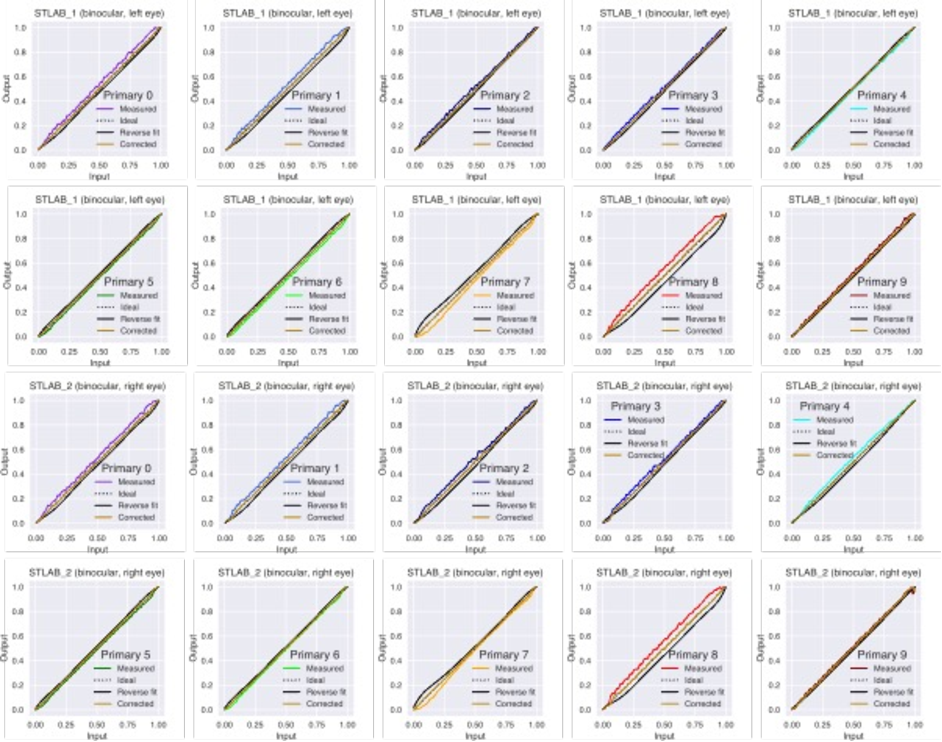
\includegraphics{Figures/SuppFig1} 

}

\caption{Linearity of primaries for each device. The calibration measures were summed (i.e., total unweighted irradiance), and the input-output relationship summarised by a 7th order polynomial reverse curve fit. By applying the coefficients of the regression, it is possible to achieve a linear output in the primaries.}\label{fig:primarylinearity}
\end{figure}

\end{document}
